\documentclass[a4paper,12pt]{article}
\usepackage[utf8]{inputenc}
\usepackage{amsmath}
\usepackage{comment}
\usepackage{graphicx}
\usepackage[left=1.5cm, right=1.5cm, top=2cm, bottom=2cm]{geometry}
\title{\textbf{COM 5120 Communication Theory}}
\author{\textbf{Midterm Exam}}
\date{November 10, 2022 \\ 
15:30 $\sim$ 17:20
}
\begin{document}
    \maketitle
    \textit{Note: }There are \textbf{7} problems with total 100 points within \textbf{3} pages, please write your answer with detail in the answer sheet.

    {\bf No credit without detail, except for question 1.  No calculator. Closed books.}

    \begin{enumerate}
    %%%%%%%%%%%%%%%%%%%%%%%%%%%%%%
        \item (13\%) 
            A transmitter transmits signal $s$ via AWGN model $r = s \,+\,n$, where $r$ is the received signal at the receiver, n is the white noise with $N(0, \sigma^2)$, which of the following is \textbf{NOT} a \textbf{sufficient statistic} with respect to the estimation of $s$ at the receiver? Assuming the same signal $s$ is transmitted 3 times. The received signals are denoted as $r_1, r_2, r_3.$ 
            % (Single choice, no derivation required)
            {\bf (Single choice, no derivation required)} 
            \\ \\
            (a) $\{r_1, r_2, r_3\}$ \\ \\
            (b) $ \sum_{i=1}^{3} r_i $ \\ \\
            (c) $ \frac{1}{2} \sum_{i=1}^{2} r_i $ \\ \\
            (d) $\{ \sum_{i=1}^{3} r_i \}^3$ \\ \\
            (e) $ \frac{1}{3} \sum_{i=1}^{3} r_i $ \\ \\
            (f) $ \frac{1}{2} \sum_{i=1}^{3} r_i $ \\
    %%%%%%%%%%%%%%%%%%%%%%%%%%%%%%
        \item (15\%) 
            We observed $N$ i.i.d. Bernoulli experiments, $x[n]$, $n = 1 \sim N$, with $P_r\{x[n] = 1\} = p$, $P_r\{x[n] = 0\} = 1 - p$. Derive and find the \textbf{maximum likelihood estimator} of $p$.  \\
    %%%%%%%%%%%%%%%%%%%%%%%%%%%%%    
        \item(15\%) 
            Let $X(t)$ denote a (real, zero-mean, WSS) bandpass process with autocorrelation function $R_X(\tau)$ and power spectral density $S_X(f)$, where $S_X(0) = 0$, and let $\hat{X}(t)$ denote the Hilbert transform of $X(t)$. 
            Then $\hat{X}(t)$ can be viewed as the output of a filter, with impulse response $\frac{1}{\pi t}$ and transfer function $- j \text{sgn}(f)$, whose input is $X(t)$. 
            Recall that when $X(t)$ passes through a system with transfer function $H(f)$ and the output is $Y(t)$, we have $S_Y(f) = S_X(f)|H(t)|^2$ and $S_{XY}(f) = S_X(f)H^*(f)$. \\
            (a) Prove that $R_{\hat{X}}(\tau) = R_{X}(\tau)$ \\
            (b) Prove that $R_{X\hat{X}}(\tau) = - \hat{R}_{X}(\tau)$ \\
            (c) If $Z(t) = X(t) + j \hat{X}(t)$, determine $S_Z(f)$ in terms of $S_X(f)$ \\
            % (d) Define $X_{l}(t) = Z(t)e^{- j2 \pi f_{0} t}$.  Show that $X_{l}(t)$ is a lowpass WSS random process, and determine $S_{X_l}(f)$. From the expression for $S_{X_l}(f)$, derive an expression for $R_{X_l}(\tau)$ \\
            \newpage
    %%%%%%%%%%%%%%%%%%%%%%%%%%%%%%
        \item (14\%) 
            Consider the three waveforms $f_n(t)$ shown in Figure 1. \\ 
            (a) Show that these waveforms are \textbf{orthonormal}. \\ 
            (b) Express the waveform $x(t)$  as a \textbf{linear combination} of $f_n(t)$, $n = 1, 2, 3$ if 
            $$x = \left\{ 
            \begin{aligned}
                -2, \; 0 \leq t < 1 \\
                 6, \; 1 \leq t < 3 \\ 
                 4, \; 3 \leq t < 4 \\
            \end{aligned}
            \right.
            $$ \\
            and determine the \textbf{weighting coefficients}.
            \begin{figure}[h]
            	\centering
            	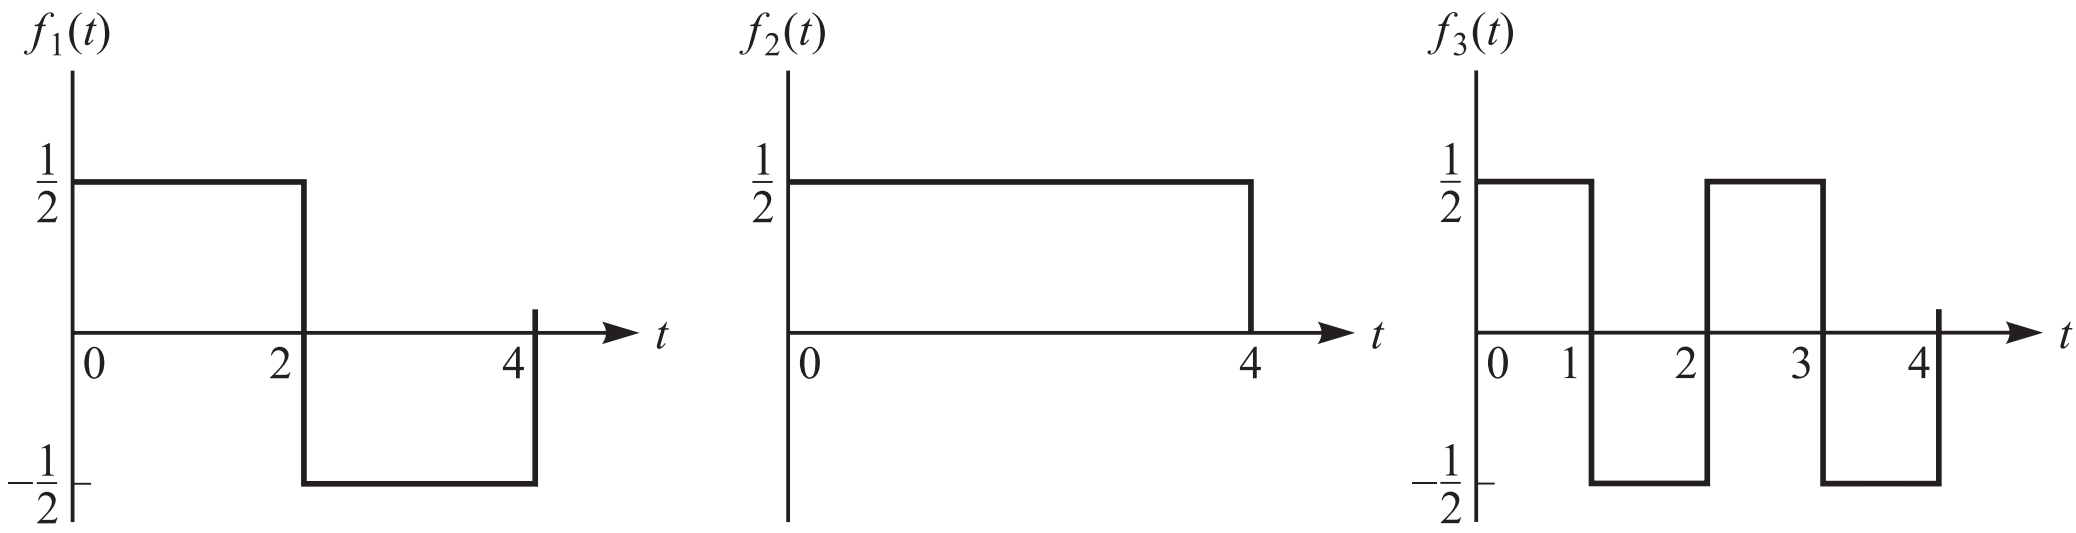
\includegraphics[scale=0.3]{Mid_fig1.png}
            	\caption{three waveforms $f_1(t)$, $f_2(t)$, $f_3(t)$}
            % 	\label{fig}
            \end{figure}
            % \newpage
    %%%%%%%%%%%%%%%%%%%%%%%%%%%%%%
        \item (14\%) 
            Consider the octal signal point constellations shown in Figure 2. \\ 
            (a) The nearest-neighbor signal points in the 8-QAM signal constellation are separated in distance by $A$ units. Determine the \textbf{radii} $a$ and $b$ of the inner and outer circles, respectively. \\
            (b) The adjacent signal points in the 8-PSK are separated by a distance of $A$ units. Determine the \textbf{radius} $r$ of the circle. \\
            \begin{figure}[h]
            	\centering
            	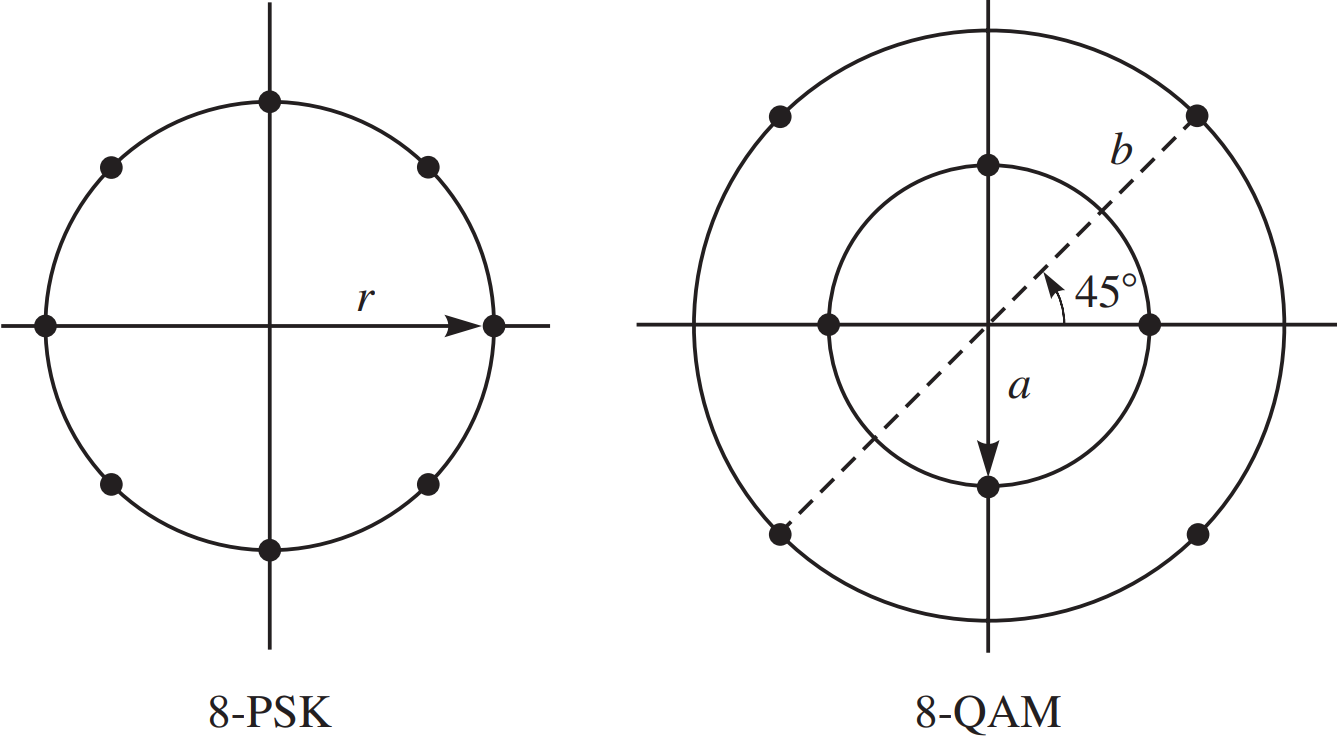
\includegraphics[scale=0.4]{Mid_fig2.png}
            	\caption{8-PSK and 8-QAM}
            % 	\label{fig}
            \end{figure}
            \newpage
            
    %%%%%%%%%%%%%%%%%%%%%%%%%%%%%%%%%%%%%%%%%%%%%%    
        \item(14\%) 
            A binary digital communication system employs the signals \\ 
            $$s_0(t) = 0, \; 0 \leq t \leq T$$
            $$s_1(t) = A, \; 0 \leq t \leq T$$
            for transmitting the information. This is called \emph{on-off signaling}. The demodulator crosscorrelates the received signal $r(t)$ with $s(t)$ and samples the output of the correlator at $t + T$. \\
            (a) Determine the \textbf{optimum detector} for an AWGN channel and the \textbf{optimum threshold}, assuming that the signals are equally probable. \\ 
            \textbf{Given that the correlation type demodulator employes a filter:} \\ 
            $$f(t) = \left\{ 
            \begin{aligned}
                \frac{1}{\sqrt{T}}, \; 0 \leq t < T \\
                 0, \; otherwise \\ 
            \end{aligned}
            \right.
            $$ \\
            (b) Determine the \textbf{probability of error} as a function of the SNR. How does on-off signaling compare with antipodal signaling? \\
     %%%%%%%%%%%%%%%%%%%%%%%%%%%%%%%%%%%%%%%%%%%   
        \item(15\%) 
            Consider a signal detector with an input $$r = \pm A + n$$ where $+A$ and $-A$ occur with equal probability and the noise variable $n$ is characterized by the (Laplacian) PDF shown in Figure 3, where $p(n) = \frac{1}{\sqrt{2\sigma}}e^{-|n|\sqrt{\frac{2}{\sigma}}}$.
            % (a) 
            Determine the \textbf{probability of error} as a function of the parameters $A$ and $\sigma$. \\
            % (b) Determine the \textbf{SNR} required to achieve an error probability of $10^{-5}$. How does the SNR compare with the result for a Gaussian PDF? \\
            \begin{figure}[h]
            	\centering
            	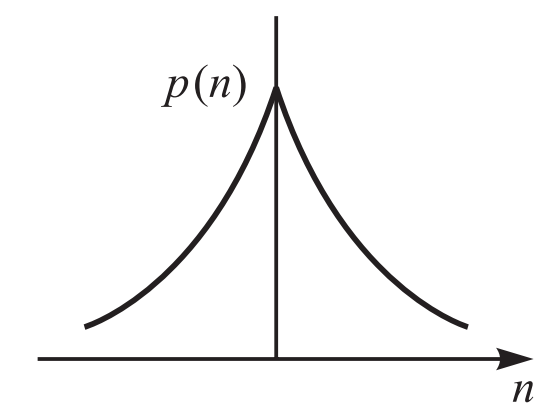
\includegraphics[scale=0.4]{Mid_fig4.png}
            	\caption{Laplacian PDF, $p(n) = \frac{1}{\sqrt{2\sigma}}e^{-|n|\sqrt{\frac{2}{\sigma}}}$}
            % 	\label{fig}
            \end{figure}
    \end{enumerate}
    \rule{\textwidth}{0.4pt}
\end{document}


